% Seminar 0: Introduction: components and exponential smoothing
% Time Series Analysis -- Bachelor's programmes Economic Informatics and Economic Cybernetics, Bucharest University of Economic Studies
% GENERATED by latex/build_seminar0.py -- edit the generator, not this file.
% Student version by default; the instructor version is the *_solutions.tex wrapper.
\makeatletter\@ifundefined{ifsolutions}{\expandafter\newif\csname ifsolutions\endcsname}{}\makeatother

\newcommand{\coursename}{Time Series Analysis}
% Preambul comun TSA -- Serii de timp / Time Series Analysis (Beamer, 16:9)
% Același design ca MFM și SFM (preluat din SFM, 5 octombrie 2026). Înainte de % Preambul comun TSA -- Serii de timp / Time Series Analysis (Beamer, 16:9)
% Același design ca MFM și SFM (preluat din SFM, 5 octombrie 2026). Înainte de % Preambul comun TSA -- Serii de timp / Time Series Analysis (Beamer, 16:9)
% Același design ca MFM și SFM (preluat din SFM, 5 octombrie 2026). Înainte de \input{../../latex/preamble} se definește
%   \newcommand{\coursename}{Time Series Analysis}      (EN)
%   \newcommand{\coursename}{Serii de timp}       (RO)  și  \def\tsalang{ro}
% Fișierele .tex se află în EN/Courses, EN/Seminars, RO/Cursuri, RO/Seminarii (două niveluri sub rădăcină).
% Deck-urile sînt generate de latex/build_chapterN.py / build_seminarN.py (vezi latex/tsa_build.py).

\documentclass[9pt, aspectratio=169, t]{beamer}
\providecommand{\coursename}{Time Series Analysis}

% Ensure content fits on slides
\setbeamersize{text margin left=8mm, text margin right=8mm}
% Smaller institute font (title page)
\setbeamerfont{institute}{size=\footnotesize}

%=============================================================================
% THEME AND STYLE CONFIGURATION
%=============================================================================
\usetheme{default}
% Using default theme for clean header/footer control

% Color Palette (matching Redispatch PDF)
\definecolor{MainBlue}{RGB}{26, 58, 110}
\definecolor{AccentBlue}{RGB}{26, 58, 110}
\definecolor{IDAred}{RGB}{205, 0, 0}
\definecolor{DarkGray}{RGB}{51, 51, 51}
\definecolor{MediumGray}{RGB}{128, 128, 128}
\definecolor{LightGray}{RGB}{248, 248, 248}
\definecolor{VeryLightGray}{RGB}{235, 235, 235}
\definecolor{KeynoteGray}{RGB}{218, 218, 218}
\definecolor{SectionGray}{RGB}{120, 120, 120}
\definecolor{FooterGray}{RGB}{100, 100, 100}
\definecolor{Crimson}{RGB}{220, 53, 69}
\definecolor{Forest}{RGB}{46, 125, 50}
\definecolor{Amber}{RGB}{181, 133, 63}
\definecolor{Orange}{RGB}{230, 126, 34}
\definecolor{Purple}{RGB}{142, 68, 173}

% Gradient background (exact Keynote 315° gradient: white to RGB 218,218,218)
\setbeamertemplate{background}{%
    \begin{tikzpicture}[remember picture, overlay]
        \shade[shading=axis, shading angle=315,
        top color=white, bottom color=KeynoteGray]
        (current page.south west) rectangle (current page.north east);
    \end{tikzpicture}%
}
% Fallback solid color for compatibility
\setbeamercolor{background canvas}{bg=}

\setbeamercolor{palette primary}{bg=MainBlue, fg=white}
\setbeamercolor{palette secondary}{bg=MainBlue!85, fg=white}
\setbeamercolor{palette tertiary}{bg=MainBlue!70, fg=white}
\setbeamercolor{structure}{fg=MainBlue}
\setbeamercolor{title}{fg=IDAred}
\setbeamercolor{frametitle}{fg=IDAred, bg=}
\setbeamercolor{block title}{bg=MainBlue, fg=white}
\setbeamercolor{block body}{bg=VeryLightGray, fg=DarkGray}
\setbeamercolor{block title alerted}{bg=Crimson, fg=white}
\setbeamercolor{block body alerted}{bg=Crimson!8, fg=DarkGray}
\setbeamercolor{block title example}{bg=Forest, fg=white}
\setbeamercolor{block body example}{bg=Forest!8, fg=DarkGray}
\setbeamercolor{item}{fg=MainBlue}

% Footer colors (override Madrid theme blue)
\setbeamercolor{author in head/foot}{fg=FooterGray, bg=}
\setbeamercolor{title in head/foot}{fg=FooterGray, bg=}
\setbeamercolor{date in head/foot}{fg=FooterGray, bg=}
\setbeamercolor{section in head/foot}{fg=FooterGray, bg=}
\setbeamercolor{subsection in head/foot}{fg=FooterGray, bg=}

% Bullet styles (apply everywhere including blocks)
\setbeamertemplate{itemize item}{\color{MainBlue}$\boxdot$}
\setbeamertemplate{itemize subitem}{\color{MainBlue}$\blacktriangleright$}
\setbeamertemplate{itemize subsubitem}{\color{MainBlue}\tiny$\bullet$}
\setbeamertemplate{itemize/enumerate body begin}{\normalsize}
\setbeamertemplate{itemize/enumerate subbody begin}{\normalsize}

% Item spacing - compact style
\setlength{\leftmargini}{10pt}       % Level 1: minimal indent
\setlength{\leftmarginii}{10pt}      % Level 2: minimal additional indent
% Compact list spacing (zero extra space before/after lists in blocks)
\makeatletter
\def\@listi{\leftmargin\leftmargini \topsep 0pt \parsep 0pt \itemsep 0pt}
\def\@listii{\leftmargin\leftmarginii \topsep 0pt \parsep 0pt \itemsep 0pt}
\makeatother

\setbeamertemplate{navigation symbols}{}

%=============================================================================
% CUSTOM HEADLINE
%=============================================================================
\setbeamertemplate{headline}{%
    \vskip10pt%
    \hbox to \paperwidth{%
        \hskip0.5cm%
        {\small\color{FooterGray}\renewcommand{\hyperlink}[2]{##2}\insertsectionhead}%
        \hfill%
        \textcolor{FooterGray}{\small\insertframenumber}%
        \hskip0.5cm%
    }%
    \vskip4pt%
    {\color{FooterGray}\hrule height 0.4pt}%
}

%=============================================================================
% CUSTOM FOOTER
%=============================================================================
\usepackage{fontawesome5}

\setbeamertemplate{footline}{%
    {\color{FooterGray}\hrule height 0.4pt}%
    \vskip4pt%
    \hbox to \paperwidth{%
        \hskip0.5cm%
        \textcolor{FooterGray}{\small\coursename}%
        \hfill%
        \raisebox{-0.1em}{%
            \begin{tikzpicture}[x=0.08em, y=0.08em, line width=0.4pt]
                \draw[FooterGray] (0,3) -- (1,4) -- (2,3.5) -- (3,5) -- (4,4) -- (5,6) -- (6,5.5) -- (7,4) -- (8,5) -- (9,7) -- (10,6) -- (11,5) -- (12,6.5) -- (13,8) -- (14,7) -- (15,6) -- (16,7.5) -- (17,9) -- (18,8) -- (19,7) -- (20,8.5) -- (21,10) -- (22,9) -- (23,8) -- (24,9.5);
            \end{tikzpicture}%
        }%
        \hskip0.5cm%
    }%
    \vskip6pt%
}

%=============================================================================
% PACKAGES
%=============================================================================
\usepackage[utf8]{inputenc}
\DeclareUnicodeCharacter{03B1}{\ensuremath{\alpha}}
\usepackage[T1]{fontenc}
\usepackage{amsmath, amssymb, amsthm}
\usepackage{mathtools}
\usepackage{bm}
\usepackage{tikz}
\usetikzlibrary{arrows.meta, positioning, shapes, calc, decorations.pathreplacing, shadings}
\usepackage{booktabs}
\usepackage{multirow}
\usepackage{array}
\usepackage{graphicx}
\usepackage{animate}
\usepackage{hyperref}
\usepackage{colortbl}
\usepackage{listings}
\lstset{language=Python, basicstyle=\ttfamily\scriptsize, keywordstyle=\color{MainBlue}\bfseries,
  commentstyle=\color{Forest}, stringstyle=\color{Crimson}, breaklines=true,
  frame=none, backgroundcolor=\color{VeryLightGray}, xleftmargin=2mm}
\hypersetup{colorlinks=true, linkcolor=MainBlue, urlcolor=MainBlue}
\graphicspath{{../../logos/}{../../charts/}{../../photos/}}
\usepackage{xcolor}
\hfuzz=2pt  % Suppress tiny overfull warnings (<2pt)
\vfuzz=2pt  % Suppress tiny vertical overfull warnings (<2pt)
% \mathrm in the sans-serif family of the slides (beamer resets \mathrm to the serif family at \begin{document};
% this hook runs after beamer's, so WN, Var, RMSE, ... in formulas match the surrounding text)
% Bold vectors and matrices in the same sans-serif family: \mathbf{A} in sans bold (beamer's own \mathbf came out in
% medium weight), and the bold upright Greek capitals of \boldsymbol / \bm (\bSigma, \bPhi, \boldsymbol{\Theta}) in
% cmss bold: bm.sty fixes its "boldoperators" font when it is loaded (serif cmbx), before beamer switches the
% operators to cmss, so it is reset here.
\AtBeginDocument{%
  \SetMathAlphabet{\mathrm}{normal}{\encodingdefault}{\sfdefault}{\mddefault}{n}%
  \SetMathAlphabet{\mathrm}{bold}{\encodingdefault}{\sfdefault}{bx}{n}%
  \SetMathAlphabet{\mathbf}{normal}{\encodingdefault}{\sfdefault}{bx}{n}%
  \SetMathAlphabet{\mathbf}{bold}{\encodingdefault}{\sfdefault}{bx}{n}%
  \SetSymbolFont{boldoperators}{normal}{OT1}{cmss}{bx}{n}%
  \SetSymbolFont{boldoperators}{bold}{OT1}{cmss}{bx}{n}}

%=============================================================================
% QUANTLET COMMANDS
%   \quantlet{<displayed name>}{<url>}       (generic, compatible with the older TSA decks)
%   \tsaquantlet{Ch_05}{TSA_ch5_garch}       -> https://github.com/danpele/Time-Series-Analysis/tree/main/Quantlets/Ch_05/TSA_ch5_garch
%   \qlurl{<folder>} is defined per chapter by the generator (Quantlets/Ch_NN/<folder>)
%=============================================================================
\newcommand{\tsarepo}{https://github.com/danpele/Time-Series-Analysis}
\newcommand{\tsaqlbase}{https://github.com/danpele/Time-Series-Analysis/tree/main/Quantlets}
\newcommand{\quantlet}[2]{%
    \hfill\href{#2}{%
        \raisebox{-0.15em}{
\includegraphics[height=0.7em]{ql_logo.png}}%
        \textcolor{MainBlue}{\tiny\ #1}%
    }%
}
\newcommand{\tsaquantlet}[2]{\quantlet{\detokenize{#2}}{\tsaqlbase/#1/#2}}

%=============================================================================
% NOTEBOOKS (Google Colab)
%   \colaburl{notebooks/EN/chapter5_seminar_notebook.ipynb} -> the Colab link of a file in the TSA repo
%   \nb: the chapter notebook (each seminar deck redefines it with \renewcommand)
%=============================================================================
\newcommand{\colaburl}[1]{https://colab.research.google.com/github/danpele/Time-Series-Analysis/blob/main/#1}
\newcommand{\nb}{https://colab.research.google.com/github/danpele/Time-Series-Analysis/tree/main/notebooks/EN}
\newcommand{\nbname}{notebooks/EN}

%=============================================================================
% SLIDE HELPERS (used by the generators; the same as in MFM)
%=============================================================================
% local font size for list bodies (the preamble forces \normalsize)
\newcommand{\itemsize}[1]{\setbeamertemplate{itemize/enumerate body begin}{#1}\setbeamertemplate{itemize/enumerate subbody begin}{#1}}
\newcommand{\intitle}[1]{{\hypersetup{urlcolor=white}#1}}   % white links inside coloured title bars
\newcommand{\imgcap}[1]{{\scriptsize #1}\\[0.5mm]}          % caption under a photo
\newcommand{\imgcredit}[2]{{\tiny\color{FooterGray}\href{#1}{#2}}}   % image credit: source URL, author/licence
\newcommand{\aiprompt}[1]{{\ttfamily\color{MainBlue}#1}}     % a prompt to an AI assistant

%=============================================================================
% SEMINARS: student version by default; the instructor wrapper *_solutions.tex sets \solutionstrue
%=============================================================================
\makeatletter\@ifundefined{ifsolutions}{\expandafter\newif\csname ifsolutions\endcsname}{}\makeatother
\newcommand{\solonly}[1]{\ifsolutions #1\fi}
\newcommand{\propsub}{\ifsolutions\else\framesubtitle{\ifdefined\tsalang Rezolvarea se discută la seminar\else Solution discussed in class\fi}\fi}

%=============================================================================
% APPENDIX AND CHAPTER LINKS (latex/appendix_links.py writes the calls; it also re-declares these
% macros before \begin{document}, so the decks compile with or without this preamble block)
%=============================================================================
\providecommand{\tsaapplink}[3]{\hypertarget{#2}{}\hyperlink{#1}{\beamergotobutton{#3}}}
\providecommand{\tsaappback}[2]{\begin{tikzpicture}[remember picture,overlay]\node[anchor=south east] at ([xshift=-3mm,yshift=7mm]current page.south east){\hyperlink{#1}{\beamerreturnbutton{#2}}};\end{tikzpicture}}
\providecommand{\tsachlink}[2]{\href{#1}{#2}}
\providecommand{\tsachlinkt}[2]{\href{#1}{\usebeamercolor[fg]{frametitle}#2}}

%=============================================================================
% QUANTINAR COMMAND: link către un curs Quantinar (subiecte avansate)
%=============================================================================
\newcommand{\quantinar}[2]{%
    \href{#2}{%
        \raisebox{-0.15em}{
\includegraphics[height=0.8em]{qr_logo.png}}%
        \textcolor{MainBlue}{\scriptsize\ #1}%
    }%
}

%=============================================================================
% CUSTOM TITLE PAGE
%=============================================================================
\defbeamertemplate*{title page}{hybrid}[1][]
{
    \vspace{0.2cm}
    % Logos row - top header (with clickable links)
    \begin{center}
        \href{https://www.ase.ro}{
\includegraphics[height=1.0cm]{ase_logo.png}}\hspace{0.3cm}%
        \href{https://theida.net}{
\includegraphics[height=1.0cm]{ida_logo.png}}\hspace{0.3cm}%
        \href{https://blockchain-research-center.com}{
\includegraphics[height=1.0cm]{brc_logo.png}}\hspace{0.3cm}%
        \href{https://www.ai4efin.ase.ro}{
\includegraphics[height=1.0cm]{ai4efin_logo.png}}\hspace{0.3cm}%
        \href{https://ipe.ro/new}{
\includegraphics[height=1.0cm]{acad_logo.png}}\hspace{0.3cm}%
        \href{https://www.digital-finance-msca.com}{
\includegraphics[height=1.0cm]{msca_logo.png}}%
    \end{center}

    \vspace{0.6cm}

    % Main title with Q logos on sides (with clickable links)
    \begin{center}
        \begin{minipage}{0.1\textwidth}
            \centering
            \href{https://quantlet.com}{
\includegraphics[height=1.1cm]{ql_logo.png}}
        \end{minipage}%
        \begin{minipage}{0.78\textwidth}
            \centering
            {\LARGE\bfseries\usebeamercolor[fg]{title}\inserttitle}

            \vspace{0.3cm}

            {\usebeamerfont{subtitle}\usebeamercolor[fg]{title}\insertsubtitle}
        \end{minipage}%
        \begin{minipage}{0.1\textwidth}
            \centering
            \href{https://quantinar.com}{
\includegraphics[height=1.1cm]{qr_logo.png}}
        \end{minipage}
    \end{center}

    \vspace{0.6cm}

    % Authors (left aligned)
    \hspace{0.5cm}{\usebeamerfont{author}\insertauthor}

    \vspace{0.3cm}

    % Institute/Affiliations (left aligned)
    \hspace{0.5cm}\begin{minipage}[t]{0.9\textwidth}
        \raggedright\small\insertinstitute
    \end{minipage}
}

%=============================================================================
% THEOREM ENVIRONMENTS
%=============================================================================
\theoremstyle{definition}
\setbeamertemplate{theorems}[numbered]
\ifdefined\tsalang
\newtheorem{defn}{Definiție}
\newtheorem{thm}{Teoremă}
\newtheorem{prop}{Propoziție}
\newtheorem{rmk}{Observație}
\else
\newtheorem{defn}{Definition}
\newtheorem{thm}{Theorem}
\newtheorem{prop}{Proposition}
\newtheorem{rmk}{Remark}
\fi

%=============================================================================
% CENTRED MINIPAGE (no extra vertical space)
%=============================================================================
\newenvironment{cminipage}[1]{%
    \par\noindent\hfill\begin{minipage}{#1}\ignorespaces
}{%
    \end{minipage}\hfill\null\par
}

%=============================================================================
% CUSTOM COMMANDS
%=============================================================================
\newcommand{\E}{\mathbb{E}}
\newcommand{\Var}{\text{Var}}
\newcommand{\Cov}{\text{Cov}}
\newcommand{\Corr}{\text{Corr}}
\newcommand{\R}{\mathbb{R}}
\newcommand{\N}{\mathbb{N}}
\newcommand{\Z}{\mathbb{Z}}
\newcommand{\B}{\mathbf{B}}
\newcommand{\imark}{\textcolor{MainBlue}{\textbullet}}
\newcommand{\RMSE}{\text{RMSE}}
\newcommand{\MAE}{\text{MAE}}
\newcommand{\MAPE}{\text{MAPE}}

% Boldface vector/matrix commands (VAR, VECM, state space; also used by the older TSA decks)
\newcommand{\bY}{\mathbf{Y}}
\newcommand{\bX}{\mathbf{X}}
\newcommand{\bA}{\mathbf{A}}
\newcommand{\bB}{\mathbf{B}}
\newcommand{\bepsilon}{\boldsymbol{\varepsilon}}
\newcommand{\bSigma}{\boldsymbol{\Sigma}}
\newcommand{\bPhi}{\boldsymbol{\Phi}}
\newcommand{\bGamma}{\boldsymbol{\Gamma}}
\newcommand{\bPi}{\boldsymbol{\Pi}}
\newcommand{\bc}{\mathbf{c}}
\newcommand{\balpha}{\boldsymbol{\alpha}}
\newcommand{\bbeta}{\boldsymbol{\beta}}
\newcommand{\bvarepsilon}{\boldsymbol{\varepsilon}}

% Legacy seminar marks (older TSA seminar decks)
\newcommand{\correct}{\textcolor{Forest}{\checkmark}}
\newcommand{\incorrect}{\textcolor{Crimson}{\texttimes}}
 se definește
%   \newcommand{\coursename}{Time Series Analysis}      (EN)
%   \newcommand{\coursename}{Serii de timp}       (RO)  și  \def\tsalang{ro}
% Fișierele .tex se află în EN/Courses, EN/Seminars, RO/Cursuri, RO/Seminarii (două niveluri sub rădăcină).
% Deck-urile sînt generate de latex/build_chapterN.py / build_seminarN.py (vezi latex/tsa_build.py).

\documentclass[9pt, aspectratio=169, t]{beamer}
\providecommand{\coursename}{Time Series Analysis}

% Ensure content fits on slides
\setbeamersize{text margin left=8mm, text margin right=8mm}
% Smaller institute font (title page)
\setbeamerfont{institute}{size=\footnotesize}

%=============================================================================
% THEME AND STYLE CONFIGURATION
%=============================================================================
\usetheme{default}
% Using default theme for clean header/footer control

% Color Palette (matching Redispatch PDF)
\definecolor{MainBlue}{RGB}{26, 58, 110}
\definecolor{AccentBlue}{RGB}{26, 58, 110}
\definecolor{IDAred}{RGB}{205, 0, 0}
\definecolor{DarkGray}{RGB}{51, 51, 51}
\definecolor{MediumGray}{RGB}{128, 128, 128}
\definecolor{LightGray}{RGB}{248, 248, 248}
\definecolor{VeryLightGray}{RGB}{235, 235, 235}
\definecolor{KeynoteGray}{RGB}{218, 218, 218}
\definecolor{SectionGray}{RGB}{120, 120, 120}
\definecolor{FooterGray}{RGB}{100, 100, 100}
\definecolor{Crimson}{RGB}{220, 53, 69}
\definecolor{Forest}{RGB}{46, 125, 50}
\definecolor{Amber}{RGB}{181, 133, 63}
\definecolor{Orange}{RGB}{230, 126, 34}
\definecolor{Purple}{RGB}{142, 68, 173}

% Gradient background (exact Keynote 315° gradient: white to RGB 218,218,218)
\setbeamertemplate{background}{%
    \begin{tikzpicture}[remember picture, overlay]
        \shade[shading=axis, shading angle=315,
        top color=white, bottom color=KeynoteGray]
        (current page.south west) rectangle (current page.north east);
    \end{tikzpicture}%
}
% Fallback solid color for compatibility
\setbeamercolor{background canvas}{bg=}

\setbeamercolor{palette primary}{bg=MainBlue, fg=white}
\setbeamercolor{palette secondary}{bg=MainBlue!85, fg=white}
\setbeamercolor{palette tertiary}{bg=MainBlue!70, fg=white}
\setbeamercolor{structure}{fg=MainBlue}
\setbeamercolor{title}{fg=IDAred}
\setbeamercolor{frametitle}{fg=IDAred, bg=}
\setbeamercolor{block title}{bg=MainBlue, fg=white}
\setbeamercolor{block body}{bg=VeryLightGray, fg=DarkGray}
\setbeamercolor{block title alerted}{bg=Crimson, fg=white}
\setbeamercolor{block body alerted}{bg=Crimson!8, fg=DarkGray}
\setbeamercolor{block title example}{bg=Forest, fg=white}
\setbeamercolor{block body example}{bg=Forest!8, fg=DarkGray}
\setbeamercolor{item}{fg=MainBlue}

% Footer colors (override Madrid theme blue)
\setbeamercolor{author in head/foot}{fg=FooterGray, bg=}
\setbeamercolor{title in head/foot}{fg=FooterGray, bg=}
\setbeamercolor{date in head/foot}{fg=FooterGray, bg=}
\setbeamercolor{section in head/foot}{fg=FooterGray, bg=}
\setbeamercolor{subsection in head/foot}{fg=FooterGray, bg=}

% Bullet styles (apply everywhere including blocks)
\setbeamertemplate{itemize item}{\color{MainBlue}$\boxdot$}
\setbeamertemplate{itemize subitem}{\color{MainBlue}$\blacktriangleright$}
\setbeamertemplate{itemize subsubitem}{\color{MainBlue}\tiny$\bullet$}
\setbeamertemplate{itemize/enumerate body begin}{\normalsize}
\setbeamertemplate{itemize/enumerate subbody begin}{\normalsize}

% Item spacing - compact style
\setlength{\leftmargini}{10pt}       % Level 1: minimal indent
\setlength{\leftmarginii}{10pt}      % Level 2: minimal additional indent
% Compact list spacing (zero extra space before/after lists in blocks)
\makeatletter
\def\@listi{\leftmargin\leftmargini \topsep 0pt \parsep 0pt \itemsep 0pt}
\def\@listii{\leftmargin\leftmarginii \topsep 0pt \parsep 0pt \itemsep 0pt}
\makeatother

\setbeamertemplate{navigation symbols}{}

%=============================================================================
% CUSTOM HEADLINE
%=============================================================================
\setbeamertemplate{headline}{%
    \vskip10pt%
    \hbox to \paperwidth{%
        \hskip0.5cm%
        {\small\color{FooterGray}\renewcommand{\hyperlink}[2]{##2}\insertsectionhead}%
        \hfill%
        \textcolor{FooterGray}{\small\insertframenumber}%
        \hskip0.5cm%
    }%
    \vskip4pt%
    {\color{FooterGray}\hrule height 0.4pt}%
}

%=============================================================================
% CUSTOM FOOTER
%=============================================================================
\usepackage{fontawesome5}

\setbeamertemplate{footline}{%
    {\color{FooterGray}\hrule height 0.4pt}%
    \vskip4pt%
    \hbox to \paperwidth{%
        \hskip0.5cm%
        \textcolor{FooterGray}{\small\coursename}%
        \hfill%
        \raisebox{-0.1em}{%
            \begin{tikzpicture}[x=0.08em, y=0.08em, line width=0.4pt]
                \draw[FooterGray] (0,3) -- (1,4) -- (2,3.5) -- (3,5) -- (4,4) -- (5,6) -- (6,5.5) -- (7,4) -- (8,5) -- (9,7) -- (10,6) -- (11,5) -- (12,6.5) -- (13,8) -- (14,7) -- (15,6) -- (16,7.5) -- (17,9) -- (18,8) -- (19,7) -- (20,8.5) -- (21,10) -- (22,9) -- (23,8) -- (24,9.5);
            \end{tikzpicture}%
        }%
        \hskip0.5cm%
    }%
    \vskip6pt%
}

%=============================================================================
% PACKAGES
%=============================================================================
\usepackage[utf8]{inputenc}
\DeclareUnicodeCharacter{03B1}{\ensuremath{\alpha}}
\usepackage[T1]{fontenc}
\usepackage{amsmath, amssymb, amsthm}
\usepackage{mathtools}
\usepackage{bm}
\usepackage{tikz}
\usetikzlibrary{arrows.meta, positioning, shapes, calc, decorations.pathreplacing, shadings}
\usepackage{booktabs}
\usepackage{multirow}
\usepackage{array}
\usepackage{graphicx}
\usepackage{animate}
\usepackage{hyperref}
\usepackage{colortbl}
\usepackage{listings}
\lstset{language=Python, basicstyle=\ttfamily\scriptsize, keywordstyle=\color{MainBlue}\bfseries,
  commentstyle=\color{Forest}, stringstyle=\color{Crimson}, breaklines=true,
  frame=none, backgroundcolor=\color{VeryLightGray}, xleftmargin=2mm}
\hypersetup{colorlinks=true, linkcolor=MainBlue, urlcolor=MainBlue}
\graphicspath{{../../logos/}{../../charts/}{../../photos/}}
\usepackage{xcolor}
\hfuzz=2pt  % Suppress tiny overfull warnings (<2pt)
\vfuzz=2pt  % Suppress tiny vertical overfull warnings (<2pt)
% \mathrm in the sans-serif family of the slides (beamer resets \mathrm to the serif family at \begin{document};
% this hook runs after beamer's, so WN, Var, RMSE, ... in formulas match the surrounding text)
% Bold vectors and matrices in the same sans-serif family: \mathbf{A} in sans bold (beamer's own \mathbf came out in
% medium weight), and the bold upright Greek capitals of \boldsymbol / \bm (\bSigma, \bPhi, \boldsymbol{\Theta}) in
% cmss bold: bm.sty fixes its "boldoperators" font when it is loaded (serif cmbx), before beamer switches the
% operators to cmss, so it is reset here.
\AtBeginDocument{%
  \SetMathAlphabet{\mathrm}{normal}{\encodingdefault}{\sfdefault}{\mddefault}{n}%
  \SetMathAlphabet{\mathrm}{bold}{\encodingdefault}{\sfdefault}{bx}{n}%
  \SetMathAlphabet{\mathbf}{normal}{\encodingdefault}{\sfdefault}{bx}{n}%
  \SetMathAlphabet{\mathbf}{bold}{\encodingdefault}{\sfdefault}{bx}{n}%
  \SetSymbolFont{boldoperators}{normal}{OT1}{cmss}{bx}{n}%
  \SetSymbolFont{boldoperators}{bold}{OT1}{cmss}{bx}{n}}

%=============================================================================
% QUANTLET COMMANDS
%   \quantlet{<displayed name>}{<url>}       (generic, compatible with the older TSA decks)
%   \tsaquantlet{Ch_05}{TSA_ch5_garch}       -> https://github.com/danpele/Time-Series-Analysis/tree/main/Quantlets/Ch_05/TSA_ch5_garch
%   \qlurl{<folder>} is defined per chapter by the generator (Quantlets/Ch_NN/<folder>)
%=============================================================================
\newcommand{\tsarepo}{https://github.com/danpele/Time-Series-Analysis}
\newcommand{\tsaqlbase}{https://github.com/danpele/Time-Series-Analysis/tree/main/Quantlets}
\newcommand{\quantlet}[2]{%
    \hfill\href{#2}{%
        \raisebox{-0.15em}{
\includegraphics[height=0.7em]{ql_logo.png}}%
        \textcolor{MainBlue}{\tiny\ #1}%
    }%
}
\newcommand{\tsaquantlet}[2]{\quantlet{\detokenize{#2}}{\tsaqlbase/#1/#2}}

%=============================================================================
% NOTEBOOKS (Google Colab)
%   \colaburl{notebooks/EN/chapter5_seminar_notebook.ipynb} -> the Colab link of a file in the TSA repo
%   \nb: the chapter notebook (each seminar deck redefines it with \renewcommand)
%=============================================================================
\newcommand{\colaburl}[1]{https://colab.research.google.com/github/danpele/Time-Series-Analysis/blob/main/#1}
\newcommand{\nb}{https://colab.research.google.com/github/danpele/Time-Series-Analysis/tree/main/notebooks/EN}
\newcommand{\nbname}{notebooks/EN}

%=============================================================================
% SLIDE HELPERS (used by the generators; the same as in MFM)
%=============================================================================
% local font size for list bodies (the preamble forces \normalsize)
\newcommand{\itemsize}[1]{\setbeamertemplate{itemize/enumerate body begin}{#1}\setbeamertemplate{itemize/enumerate subbody begin}{#1}}
\newcommand{\intitle}[1]{{\hypersetup{urlcolor=white}#1}}   % white links inside coloured title bars
\newcommand{\imgcap}[1]{{\scriptsize #1}\\[0.5mm]}          % caption under a photo
\newcommand{\imgcredit}[2]{{\tiny\color{FooterGray}\href{#1}{#2}}}   % image credit: source URL, author/licence
\newcommand{\aiprompt}[1]{{\ttfamily\color{MainBlue}#1}}     % a prompt to an AI assistant

%=============================================================================
% SEMINARS: student version by default; the instructor wrapper *_solutions.tex sets \solutionstrue
%=============================================================================
\makeatletter\@ifundefined{ifsolutions}{\expandafter\newif\csname ifsolutions\endcsname}{}\makeatother
\newcommand{\solonly}[1]{\ifsolutions #1\fi}
\newcommand{\propsub}{\ifsolutions\else\framesubtitle{\ifdefined\tsalang Rezolvarea se discută la seminar\else Solution discussed in class\fi}\fi}

%=============================================================================
% APPENDIX AND CHAPTER LINKS (latex/appendix_links.py writes the calls; it also re-declares these
% macros before \begin{document}, so the decks compile with or without this preamble block)
%=============================================================================
\providecommand{\tsaapplink}[3]{\hypertarget{#2}{}\hyperlink{#1}{\beamergotobutton{#3}}}
\providecommand{\tsaappback}[2]{\begin{tikzpicture}[remember picture,overlay]\node[anchor=south east] at ([xshift=-3mm,yshift=7mm]current page.south east){\hyperlink{#1}{\beamerreturnbutton{#2}}};\end{tikzpicture}}
\providecommand{\tsachlink}[2]{\href{#1}{#2}}
\providecommand{\tsachlinkt}[2]{\href{#1}{\usebeamercolor[fg]{frametitle}#2}}

%=============================================================================
% QUANTINAR COMMAND: link către un curs Quantinar (subiecte avansate)
%=============================================================================
\newcommand{\quantinar}[2]{%
    \href{#2}{%
        \raisebox{-0.15em}{
\includegraphics[height=0.8em]{qr_logo.png}}%
        \textcolor{MainBlue}{\scriptsize\ #1}%
    }%
}

%=============================================================================
% CUSTOM TITLE PAGE
%=============================================================================
\defbeamertemplate*{title page}{hybrid}[1][]
{
    \vspace{0.2cm}
    % Logos row - top header (with clickable links)
    \begin{center}
        \href{https://www.ase.ro}{
\includegraphics[height=1.0cm]{ase_logo.png}}\hspace{0.3cm}%
        \href{https://theida.net}{
\includegraphics[height=1.0cm]{ida_logo.png}}\hspace{0.3cm}%
        \href{https://blockchain-research-center.com}{
\includegraphics[height=1.0cm]{brc_logo.png}}\hspace{0.3cm}%
        \href{https://www.ai4efin.ase.ro}{
\includegraphics[height=1.0cm]{ai4efin_logo.png}}\hspace{0.3cm}%
        \href{https://ipe.ro/new}{
\includegraphics[height=1.0cm]{acad_logo.png}}\hspace{0.3cm}%
        \href{https://www.digital-finance-msca.com}{
\includegraphics[height=1.0cm]{msca_logo.png}}%
    \end{center}

    \vspace{0.6cm}

    % Main title with Q logos on sides (with clickable links)
    \begin{center}
        \begin{minipage}{0.1\textwidth}
            \centering
            \href{https://quantlet.com}{
\includegraphics[height=1.1cm]{ql_logo.png}}
        \end{minipage}%
        \begin{minipage}{0.78\textwidth}
            \centering
            {\LARGE\bfseries\usebeamercolor[fg]{title}\inserttitle}

            \vspace{0.3cm}

            {\usebeamerfont{subtitle}\usebeamercolor[fg]{title}\insertsubtitle}
        \end{minipage}%
        \begin{minipage}{0.1\textwidth}
            \centering
            \href{https://quantinar.com}{
\includegraphics[height=1.1cm]{qr_logo.png}}
        \end{minipage}
    \end{center}

    \vspace{0.6cm}

    % Authors (left aligned)
    \hspace{0.5cm}{\usebeamerfont{author}\insertauthor}

    \vspace{0.3cm}

    % Institute/Affiliations (left aligned)
    \hspace{0.5cm}\begin{minipage}[t]{0.9\textwidth}
        \raggedright\small\insertinstitute
    \end{minipage}
}

%=============================================================================
% THEOREM ENVIRONMENTS
%=============================================================================
\theoremstyle{definition}
\setbeamertemplate{theorems}[numbered]
\ifdefined\tsalang
\newtheorem{defn}{Definiție}
\newtheorem{thm}{Teoremă}
\newtheorem{prop}{Propoziție}
\newtheorem{rmk}{Observație}
\else
\newtheorem{defn}{Definition}
\newtheorem{thm}{Theorem}
\newtheorem{prop}{Proposition}
\newtheorem{rmk}{Remark}
\fi

%=============================================================================
% CENTRED MINIPAGE (no extra vertical space)
%=============================================================================
\newenvironment{cminipage}[1]{%
    \par\noindent\hfill\begin{minipage}{#1}\ignorespaces
}{%
    \end{minipage}\hfill\null\par
}

%=============================================================================
% CUSTOM COMMANDS
%=============================================================================
\newcommand{\E}{\mathbb{E}}
\newcommand{\Var}{\text{Var}}
\newcommand{\Cov}{\text{Cov}}
\newcommand{\Corr}{\text{Corr}}
\newcommand{\R}{\mathbb{R}}
\newcommand{\N}{\mathbb{N}}
\newcommand{\Z}{\mathbb{Z}}
\newcommand{\B}{\mathbf{B}}
\newcommand{\imark}{\textcolor{MainBlue}{\textbullet}}
\newcommand{\RMSE}{\text{RMSE}}
\newcommand{\MAE}{\text{MAE}}
\newcommand{\MAPE}{\text{MAPE}}

% Boldface vector/matrix commands (VAR, VECM, state space; also used by the older TSA decks)
\newcommand{\bY}{\mathbf{Y}}
\newcommand{\bX}{\mathbf{X}}
\newcommand{\bA}{\mathbf{A}}
\newcommand{\bB}{\mathbf{B}}
\newcommand{\bepsilon}{\boldsymbol{\varepsilon}}
\newcommand{\bSigma}{\boldsymbol{\Sigma}}
\newcommand{\bPhi}{\boldsymbol{\Phi}}
\newcommand{\bGamma}{\boldsymbol{\Gamma}}
\newcommand{\bPi}{\boldsymbol{\Pi}}
\newcommand{\bc}{\mathbf{c}}
\newcommand{\balpha}{\boldsymbol{\alpha}}
\newcommand{\bbeta}{\boldsymbol{\beta}}
\newcommand{\bvarepsilon}{\boldsymbol{\varepsilon}}

% Legacy seminar marks (older TSA seminar decks)
\newcommand{\correct}{\textcolor{Forest}{\checkmark}}
\newcommand{\incorrect}{\textcolor{Crimson}{\texttimes}}
 se definește
%   \newcommand{\coursename}{Time Series Analysis}      (EN)
%   \newcommand{\coursename}{Serii de timp}       (RO)  și  \def\tsalang{ro}
% Fișierele .tex se află în EN/Courses, EN/Seminars, RO/Cursuri, RO/Seminarii (două niveluri sub rădăcină).
% Deck-urile sînt generate de latex/build_chapterN.py / build_seminarN.py (vezi latex/tsa_build.py).

\documentclass[9pt, aspectratio=169, t]{beamer}
\providecommand{\coursename}{Time Series Analysis}

% Ensure content fits on slides
\setbeamersize{text margin left=8mm, text margin right=8mm}
% Smaller institute font (title page)
\setbeamerfont{institute}{size=\footnotesize}

%=============================================================================
% THEME AND STYLE CONFIGURATION
%=============================================================================
\usetheme{default}
% Using default theme for clean header/footer control

% Color Palette (matching Redispatch PDF)
\definecolor{MainBlue}{RGB}{26, 58, 110}
\definecolor{AccentBlue}{RGB}{26, 58, 110}
\definecolor{IDAred}{RGB}{205, 0, 0}
\definecolor{DarkGray}{RGB}{51, 51, 51}
\definecolor{MediumGray}{RGB}{128, 128, 128}
\definecolor{LightGray}{RGB}{248, 248, 248}
\definecolor{VeryLightGray}{RGB}{235, 235, 235}
\definecolor{KeynoteGray}{RGB}{218, 218, 218}
\definecolor{SectionGray}{RGB}{120, 120, 120}
\definecolor{FooterGray}{RGB}{100, 100, 100}
\definecolor{Crimson}{RGB}{220, 53, 69}
\definecolor{Forest}{RGB}{46, 125, 50}
\definecolor{Amber}{RGB}{181, 133, 63}
\definecolor{Orange}{RGB}{230, 126, 34}
\definecolor{Purple}{RGB}{142, 68, 173}

% Gradient background (exact Keynote 315° gradient: white to RGB 218,218,218)
\setbeamertemplate{background}{%
    \begin{tikzpicture}[remember picture, overlay]
        \shade[shading=axis, shading angle=315,
        top color=white, bottom color=KeynoteGray]
        (current page.south west) rectangle (current page.north east);
    \end{tikzpicture}%
}
% Fallback solid color for compatibility
\setbeamercolor{background canvas}{bg=}

\setbeamercolor{palette primary}{bg=MainBlue, fg=white}
\setbeamercolor{palette secondary}{bg=MainBlue!85, fg=white}
\setbeamercolor{palette tertiary}{bg=MainBlue!70, fg=white}
\setbeamercolor{structure}{fg=MainBlue}
\setbeamercolor{title}{fg=IDAred}
\setbeamercolor{frametitle}{fg=IDAred, bg=}
\setbeamercolor{block title}{bg=MainBlue, fg=white}
\setbeamercolor{block body}{bg=VeryLightGray, fg=DarkGray}
\setbeamercolor{block title alerted}{bg=Crimson, fg=white}
\setbeamercolor{block body alerted}{bg=Crimson!8, fg=DarkGray}
\setbeamercolor{block title example}{bg=Forest, fg=white}
\setbeamercolor{block body example}{bg=Forest!8, fg=DarkGray}
\setbeamercolor{item}{fg=MainBlue}

% Footer colors (override Madrid theme blue)
\setbeamercolor{author in head/foot}{fg=FooterGray, bg=}
\setbeamercolor{title in head/foot}{fg=FooterGray, bg=}
\setbeamercolor{date in head/foot}{fg=FooterGray, bg=}
\setbeamercolor{section in head/foot}{fg=FooterGray, bg=}
\setbeamercolor{subsection in head/foot}{fg=FooterGray, bg=}

% Bullet styles (apply everywhere including blocks)
\setbeamertemplate{itemize item}{\color{MainBlue}$\boxdot$}
\setbeamertemplate{itemize subitem}{\color{MainBlue}$\blacktriangleright$}
\setbeamertemplate{itemize subsubitem}{\color{MainBlue}\tiny$\bullet$}
\setbeamertemplate{itemize/enumerate body begin}{\normalsize}
\setbeamertemplate{itemize/enumerate subbody begin}{\normalsize}

% Item spacing - compact style
\setlength{\leftmargini}{10pt}       % Level 1: minimal indent
\setlength{\leftmarginii}{10pt}      % Level 2: minimal additional indent
% Compact list spacing (zero extra space before/after lists in blocks)
\makeatletter
\def\@listi{\leftmargin\leftmargini \topsep 0pt \parsep 0pt \itemsep 0pt}
\def\@listii{\leftmargin\leftmarginii \topsep 0pt \parsep 0pt \itemsep 0pt}
\makeatother

\setbeamertemplate{navigation symbols}{}

%=============================================================================
% CUSTOM HEADLINE
%=============================================================================
\setbeamertemplate{headline}{%
    \vskip10pt%
    \hbox to \paperwidth{%
        \hskip0.5cm%
        {\small\color{FooterGray}\renewcommand{\hyperlink}[2]{##2}\insertsectionhead}%
        \hfill%
        \textcolor{FooterGray}{\small\insertframenumber}%
        \hskip0.5cm%
    }%
    \vskip4pt%
    {\color{FooterGray}\hrule height 0.4pt}%
}

%=============================================================================
% CUSTOM FOOTER
%=============================================================================
\usepackage{fontawesome5}

\setbeamertemplate{footline}{%
    {\color{FooterGray}\hrule height 0.4pt}%
    \vskip4pt%
    \hbox to \paperwidth{%
        \hskip0.5cm%
        \textcolor{FooterGray}{\small\coursename}%
        \hfill%
        \raisebox{-0.1em}{%
            \begin{tikzpicture}[x=0.08em, y=0.08em, line width=0.4pt]
                \draw[FooterGray] (0,3) -- (1,4) -- (2,3.5) -- (3,5) -- (4,4) -- (5,6) -- (6,5.5) -- (7,4) -- (8,5) -- (9,7) -- (10,6) -- (11,5) -- (12,6.5) -- (13,8) -- (14,7) -- (15,6) -- (16,7.5) -- (17,9) -- (18,8) -- (19,7) -- (20,8.5) -- (21,10) -- (22,9) -- (23,8) -- (24,9.5);
            \end{tikzpicture}%
        }%
        \hskip0.5cm%
    }%
    \vskip6pt%
}

%=============================================================================
% PACKAGES
%=============================================================================
\usepackage[utf8]{inputenc}
\DeclareUnicodeCharacter{03B1}{\ensuremath{\alpha}}
\usepackage[T1]{fontenc}
\usepackage{amsmath, amssymb, amsthm}
\usepackage{mathtools}
\usepackage{bm}
\usepackage{tikz}
\usetikzlibrary{arrows.meta, positioning, shapes, calc, decorations.pathreplacing, shadings}
\usepackage{booktabs}
\usepackage{multirow}
\usepackage{array}
\usepackage{graphicx}
\usepackage{animate}
\usepackage{hyperref}
\usepackage{colortbl}
\usepackage{listings}
\lstset{language=Python, basicstyle=\ttfamily\scriptsize, keywordstyle=\color{MainBlue}\bfseries,
  commentstyle=\color{Forest}, stringstyle=\color{Crimson}, breaklines=true,
  frame=none, backgroundcolor=\color{VeryLightGray}, xleftmargin=2mm}
\hypersetup{colorlinks=true, linkcolor=MainBlue, urlcolor=MainBlue}
\graphicspath{{../../logos/}{../../charts/}{../../photos/}}
\usepackage{xcolor}
\hfuzz=2pt  % Suppress tiny overfull warnings (<2pt)
\vfuzz=2pt  % Suppress tiny vertical overfull warnings (<2pt)
% \mathrm in the sans-serif family of the slides (beamer resets \mathrm to the serif family at \begin{document};
% this hook runs after beamer's, so WN, Var, RMSE, ... in formulas match the surrounding text)
% Bold vectors and matrices in the same sans-serif family: \mathbf{A} in sans bold (beamer's own \mathbf came out in
% medium weight), and the bold upright Greek capitals of \boldsymbol / \bm (\bSigma, \bPhi, \boldsymbol{\Theta}) in
% cmss bold: bm.sty fixes its "boldoperators" font when it is loaded (serif cmbx), before beamer switches the
% operators to cmss, so it is reset here.
\AtBeginDocument{%
  \SetMathAlphabet{\mathrm}{normal}{\encodingdefault}{\sfdefault}{\mddefault}{n}%
  \SetMathAlphabet{\mathrm}{bold}{\encodingdefault}{\sfdefault}{bx}{n}%
  \SetMathAlphabet{\mathbf}{normal}{\encodingdefault}{\sfdefault}{bx}{n}%
  \SetMathAlphabet{\mathbf}{bold}{\encodingdefault}{\sfdefault}{bx}{n}%
  \SetSymbolFont{boldoperators}{normal}{OT1}{cmss}{bx}{n}%
  \SetSymbolFont{boldoperators}{bold}{OT1}{cmss}{bx}{n}}

%=============================================================================
% QUANTLET COMMANDS
%   \quantlet{<displayed name>}{<url>}       (generic, compatible with the older TSA decks)
%   \tsaquantlet{Ch_05}{TSA_ch5_garch}       -> https://github.com/danpele/Time-Series-Analysis/tree/main/Quantlets/Ch_05/TSA_ch5_garch
%   \qlurl{<folder>} is defined per chapter by the generator (Quantlets/Ch_NN/<folder>)
%=============================================================================
\newcommand{\tsarepo}{https://github.com/danpele/Time-Series-Analysis}
\newcommand{\tsaqlbase}{https://github.com/danpele/Time-Series-Analysis/tree/main/Quantlets}
\newcommand{\quantlet}[2]{%
    \hfill\href{#2}{%
        \raisebox{-0.15em}{
\includegraphics[height=0.7em]{ql_logo.png}}%
        \textcolor{MainBlue}{\tiny\ #1}%
    }%
}
\newcommand{\tsaquantlet}[2]{\quantlet{\detokenize{#2}}{\tsaqlbase/#1/#2}}

%=============================================================================
% NOTEBOOKS (Google Colab)
%   \colaburl{notebooks/EN/chapter5_seminar_notebook.ipynb} -> the Colab link of a file in the TSA repo
%   \nb: the chapter notebook (each seminar deck redefines it with \renewcommand)
%=============================================================================
\newcommand{\colaburl}[1]{https://colab.research.google.com/github/danpele/Time-Series-Analysis/blob/main/#1}
\newcommand{\nb}{https://colab.research.google.com/github/danpele/Time-Series-Analysis/tree/main/notebooks/EN}
\newcommand{\nbname}{notebooks/EN}

%=============================================================================
% SLIDE HELPERS (used by the generators; the same as in MFM)
%=============================================================================
% local font size for list bodies (the preamble forces \normalsize)
\newcommand{\itemsize}[1]{\setbeamertemplate{itemize/enumerate body begin}{#1}\setbeamertemplate{itemize/enumerate subbody begin}{#1}}
\newcommand{\intitle}[1]{{\hypersetup{urlcolor=white}#1}}   % white links inside coloured title bars
\newcommand{\imgcap}[1]{{\scriptsize #1}\\[0.5mm]}          % caption under a photo
\newcommand{\imgcredit}[2]{{\tiny\color{FooterGray}\href{#1}{#2}}}   % image credit: source URL, author/licence
\newcommand{\aiprompt}[1]{{\ttfamily\color{MainBlue}#1}}     % a prompt to an AI assistant

%=============================================================================
% SEMINARS: student version by default; the instructor wrapper *_solutions.tex sets \solutionstrue
%=============================================================================
\makeatletter\@ifundefined{ifsolutions}{\expandafter\newif\csname ifsolutions\endcsname}{}\makeatother
\newcommand{\solonly}[1]{\ifsolutions #1\fi}
\newcommand{\propsub}{\ifsolutions\else\framesubtitle{\ifdefined\tsalang Rezolvarea se discută la seminar\else Solution discussed in class\fi}\fi}

%=============================================================================
% APPENDIX AND CHAPTER LINKS (latex/appendix_links.py writes the calls; it also re-declares these
% macros before \begin{document}, so the decks compile with or without this preamble block)
%=============================================================================
\providecommand{\tsaapplink}[3]{\hypertarget{#2}{}\hyperlink{#1}{\beamergotobutton{#3}}}
\providecommand{\tsaappback}[2]{\begin{tikzpicture}[remember picture,overlay]\node[anchor=south east] at ([xshift=-3mm,yshift=7mm]current page.south east){\hyperlink{#1}{\beamerreturnbutton{#2}}};\end{tikzpicture}}
\providecommand{\tsachlink}[2]{\href{#1}{#2}}
\providecommand{\tsachlinkt}[2]{\href{#1}{\usebeamercolor[fg]{frametitle}#2}}

%=============================================================================
% QUANTINAR COMMAND: link către un curs Quantinar (subiecte avansate)
%=============================================================================
\newcommand{\quantinar}[2]{%
    \href{#2}{%
        \raisebox{-0.15em}{
\includegraphics[height=0.8em]{qr_logo.png}}%
        \textcolor{MainBlue}{\scriptsize\ #1}%
    }%
}

%=============================================================================
% CUSTOM TITLE PAGE
%=============================================================================
\defbeamertemplate*{title page}{hybrid}[1][]
{
    \vspace{0.2cm}
    % Logos row - top header (with clickable links)
    \begin{center}
        \href{https://www.ase.ro}{
\includegraphics[height=1.0cm]{ase_logo.png}}\hspace{0.3cm}%
        \href{https://theida.net}{
\includegraphics[height=1.0cm]{ida_logo.png}}\hspace{0.3cm}%
        \href{https://blockchain-research-center.com}{
\includegraphics[height=1.0cm]{brc_logo.png}}\hspace{0.3cm}%
        \href{https://www.ai4efin.ase.ro}{
\includegraphics[height=1.0cm]{ai4efin_logo.png}}\hspace{0.3cm}%
        \href{https://ipe.ro/new}{
\includegraphics[height=1.0cm]{acad_logo.png}}\hspace{0.3cm}%
        \href{https://www.digital-finance-msca.com}{
\includegraphics[height=1.0cm]{msca_logo.png}}%
    \end{center}

    \vspace{0.6cm}

    % Main title with Q logos on sides (with clickable links)
    \begin{center}
        \begin{minipage}{0.1\textwidth}
            \centering
            \href{https://quantlet.com}{
\includegraphics[height=1.1cm]{ql_logo.png}}
        \end{minipage}%
        \begin{minipage}{0.78\textwidth}
            \centering
            {\LARGE\bfseries\usebeamercolor[fg]{title}\inserttitle}

            \vspace{0.3cm}

            {\usebeamerfont{subtitle}\usebeamercolor[fg]{title}\insertsubtitle}
        \end{minipage}%
        \begin{minipage}{0.1\textwidth}
            \centering
            \href{https://quantinar.com}{
\includegraphics[height=1.1cm]{qr_logo.png}}
        \end{minipage}
    \end{center}

    \vspace{0.6cm}

    % Authors (left aligned)
    \hspace{0.5cm}{\usebeamerfont{author}\insertauthor}

    \vspace{0.3cm}

    % Institute/Affiliations (left aligned)
    \hspace{0.5cm}\begin{minipage}[t]{0.9\textwidth}
        \raggedright\small\insertinstitute
    \end{minipage}
}

%=============================================================================
% THEOREM ENVIRONMENTS
%=============================================================================
\theoremstyle{definition}
\setbeamertemplate{theorems}[numbered]
\ifdefined\tsalang
\newtheorem{defn}{Definiție}
\newtheorem{thm}{Teoremă}
\newtheorem{prop}{Propoziție}
\newtheorem{rmk}{Observație}
\else
\newtheorem{defn}{Definition}
\newtheorem{thm}{Theorem}
\newtheorem{prop}{Proposition}
\newtheorem{rmk}{Remark}
\fi

%=============================================================================
% CENTRED MINIPAGE (no extra vertical space)
%=============================================================================
\newenvironment{cminipage}[1]{%
    \par\noindent\hfill\begin{minipage}{#1}\ignorespaces
}{%
    \end{minipage}\hfill\null\par
}

%=============================================================================
% CUSTOM COMMANDS
%=============================================================================
\newcommand{\E}{\mathbb{E}}
\newcommand{\Var}{\text{Var}}
\newcommand{\Cov}{\text{Cov}}
\newcommand{\Corr}{\text{Corr}}
\newcommand{\R}{\mathbb{R}}
\newcommand{\N}{\mathbb{N}}
\newcommand{\Z}{\mathbb{Z}}
\newcommand{\B}{\mathbf{B}}
\newcommand{\imark}{\textcolor{MainBlue}{\textbullet}}
\newcommand{\RMSE}{\text{RMSE}}
\newcommand{\MAE}{\text{MAE}}
\newcommand{\MAPE}{\text{MAPE}}

% Boldface vector/matrix commands (VAR, VECM, state space; also used by the older TSA decks)
\newcommand{\bY}{\mathbf{Y}}
\newcommand{\bX}{\mathbf{X}}
\newcommand{\bA}{\mathbf{A}}
\newcommand{\bB}{\mathbf{B}}
\newcommand{\bepsilon}{\boldsymbol{\varepsilon}}
\newcommand{\bSigma}{\boldsymbol{\Sigma}}
\newcommand{\bPhi}{\boldsymbol{\Phi}}
\newcommand{\bGamma}{\boldsymbol{\Gamma}}
\newcommand{\bPi}{\boldsymbol{\Pi}}
\newcommand{\bc}{\mathbf{c}}
\newcommand{\balpha}{\boldsymbol{\alpha}}
\newcommand{\bbeta}{\boldsymbol{\beta}}
\newcommand{\bvarepsilon}{\boldsymbol{\varepsilon}}

% Legacy seminar marks (older TSA seminar decks)
\newcommand{\correct}{\textcolor{Forest}{\checkmark}}
\newcommand{\incorrect}{\textcolor{Crimson}{\texttimes}}


\newcommand{\qlurl}[1]{https://github.com/danpele/Time-Series-Analysis/tree/main/Quantlets/Ch_00/#1}
\renewcommand{\nb}{\colaburl{notebooks/EN/chapter0_seminar_notebook.ipynb}}
\renewcommand{\nbname}{chapter0\_seminar\_notebook.ipynb}
% left column: full width in the student version, narrower next to the solution
\newcommand{\taskw}{\ifsolutions 0.47\textwidth\else 0.96\textwidth\fi}
\newcommand{\solw}{\ifsolutions 0.49\textwidth\else 0pt\fi}

\title[Time Series Analysis]{Time Series Analysis}
\subtitle{Seminar 0: Introduction: components and exponential smoothing\ifsolutions\ (instructor version)\fi}
\author[D.T. Pele]{Daniel Traian PELE}
\institute{Bucharest University of Economic Studies\\
IDA Institute Digital Assets\\
Blockchain Research Center\\
AI4EFin Artificial Intelligence for Energy Finance\\
Romanian Academy, Institute for Economic Forecasting\\
MSCA Digital Finance}
\date{}

%=============================================================================
\providecommand{\tsaapplink}[3]{\hypertarget{#2}{}\hyperlink{#1}{\beamergotobutton{#3}}}  % APPLINKS-MACROS
\providecommand{\tsaappback}[2]{\begin{tikzpicture}[remember picture,overlay]\node[anchor=south east] at ([xshift=-3mm,yshift=7mm]current page.south east){\hyperlink{#1}{\beamerreturnbutton{#2}}};\end{tikzpicture}}  % APPLINKS-MACROS
\providecommand{\tsachlink}[2]{\href{#1}{#2}}  % APPLINKS-MACROS
\providecommand{\tsachlinkt}[2]{\href{#1}{\usebeamercolor[fg]{frametitle}#2}}  % APPLINKS-MACROS
\begin{document}
%=============================================================================

{
\setbeamertemplate{headline}{}
\setbeamertemplate{footline}{}
\begin{frame}[noframenumbering]
    \titlepage
\end{frame}
}
% BEGIN-ACRONYMS (generat de latex/acronyms.py; nu editati manual)
\begin{frame}{Acronyms used in this material}
\setbeamertemplate{itemize/enumerate body begin}{\tiny}
\begin{columns}[T]
\begin{column}{0.49\textwidth}
\begin{itemize}\setlength{\itemsep}{0pt}
    \item \textbf{ACF}: Autocorrelation Function
    \item \textbf{AI}: Artificial Intelligence
    \item \textbf{BNR}: Banca Națională a României (the National Bank of Romania)
    \item \textbf{GDP}: Gross Domestic Product
    \item \textbf{HICP}: Harmonised Index of Consumer Prices
    \item \textbf{INS}: Institutul Național de Statistică (the National Institute of Statistics (Romania))
    \item \textbf{MAE}: Mean Absolute Error
    \item \textbf{RMSE}: Root Mean Squared Error
    \item \textbf{STL}: Seasonal and Trend decomposition using Loess
\end{itemize}
\end{column}
\begin{column}{0.49\textwidth}
\end{column}
\end{columns}
\end{frame}
% END-ACRONYMS

%=============================================================================
\section{Route and Primer}
%=============================================================================

\begin{frame}{Today's Questions and Route}
\itemsize{\small}
\begin{itemize}
    \item First seminar of the course, before the \tsachlink{https://danpele.github.io/Time-Series-Analysis/EN/Courses/chapter0_introduction.pdf}{Chapter 0} lecture: everything you need is on the next slides
    \item \textbf{Questions of the seminar}
    \begin{itemize}
        \item how do we open the course notebooks and load a series?
        \item which growth rate tells us how the economy is doing?
        \item does today's value tell us anything about tomorrow's?
        \item how good is the simplest possible forecast?
    \end{itemize}
    \item \textbf{Part I}: setup, calculations on paper (A1--A3), the same ideas on real data (B1, B2)
    \item \textbf{Part II}: your turn (A4, B3, B4), a project idea (C1) and the critique of an AI answer (C2)
    \item Open the \href{\nb}{seminar notebook} in Google Colab; nothing is handed in
\end{itemize}
\end{frame}

\begin{frame}{Exercise Map}
\itemsize{\footnotesize}
\begin{center}
\footnotesize
\begin{tabular}{l>{\raggedright\arraybackslash}p{6.4cm}ll}
\toprule
\textbf{Exercise} & \textbf{Question} & \textbf{Type} & \textbf{Model} \\
\midrule
A1 & growth rates of a quarterly series & Solved & -- \\
A2 & a sample autocorrelation by hand & Solved & -- \\
A3 & naive forecasts and their errors & Solved & -- \\
B1 & Romanian GDP: which growth rate? & Solved & -- \\
B2 & EUR/RON: memory of levels and of changes & Solved & -- \\
A4 & the same calculations on new numbers & Proposed & A1--A3 \\
B3 & Romanian inflation: monthly and annual & Proposed & B1, B2 \\
B4 & electricity: naive or seasonal naive? & Proposed & A3 \\
C1 & a project idea & Open & -- \\
C2 & find the errors in an AI answer & Proposed & A1, A3, B1 \\
\bottomrule
\end{tabular}
\end{center}
\begin{itemize}
    \item \textbf{[Solved]}: full solution in the slides and the notebook, a model to follow; \textbf{[Proposed]}: you solve it, the solution is discussed in class
    \item Part A: on paper; Part B: real data, each task ending with an interpretation question; Part C: open
\end{itemize}
\end{frame}

\begin{frame}{Needed Today (1/2): Series and Growth Rates}
\itemsize{\small}
\begin{itemize}
    \item \textbf{Time series} $y_1, \ldots, y_T$: one variable observed at successive moments
    \begin{itemize}
        \item frequency: quarterly ($m = 4$ quarters a year), monthly ($m = 12$), daily
        \item unadjusted series contain \textbf{seasonality}: a pattern that repeats every $m$ periods
    \end{itemize}
    \item \textbf{Growth over one period}: $100\,(y_t / y_{t-1} - 1)$, in \%
    \begin{itemize}
        \item for quarterly data: quarter on quarter (q/q)
    \end{itemize}
    \item \textbf{Growth over a year}: $100\,(y_t / y_{t-m} - 1)$, year on year (y/y)
    \begin{itemize}
        \item compares the same season, so the seasonal pattern cancels out
    \end{itemize}
    \item \textbf{Log difference}: $100\,(\ln y_t - \ln y_{t-1}) \approx 100\,(y_t / y_{t-1} - 1)$ for small changes
    \begin{itemize}
        \item for a price, it is the \textbf{log return}
    \end{itemize}
\end{itemize}
\end{frame}

\begin{frame}{Needed Today (2/2): Autocorrelation and Naive Forecasts}
\itemsize{\footnotesize}
\begin{itemize}
    \item \textbf{Sample autocorrelation} at lag $k$
    \begin{itemize}
        \item $r_k = \dfrac{\sum_{t=k+1}^{T} (y_t - \bar y)(y_{t-k} - \bar y)}{\sum_{t=1}^{T} (y_t - \bar y)^2}$, between $-1$ and $1$
        \item ACF (autocorrelation function): $r_1, r_2, \ldots$ against $k$; band $\pm 1.96/\sqrt T$ for independent noise
    \end{itemize}
    \item \textbf{Naive forecast}: $\hat y_{T+h} = y_T$; \textbf{seasonal naive}: $\hat y_{T+h} = y_{T+h-m}$ ($h \le m$)
    \item \textbf{Training set and test set}: split by time
    \begin{itemize}
        \item forecasts are built on the training set and compared with the test set they have not seen
    \end{itemize}
    \item \textbf{Errors} $e = y - \hat y$ on the test set
    \begin{itemize}
        \item MAE (mean absolute error) $= \frac1h \sum |e|$; RMSE (root mean squared error) $= \sqrt{\frac1h \sum e^2}$
    \end{itemize}
\end{itemize}
\end{frame}

\begin{frame}{Data Used Today}
\itemsize{\footnotesize}
\begin{center}
\footnotesize
\begin{tabular}{>{\raggedright\arraybackslash}p{2.8cm}>{\raggedright\arraybackslash}p{2.8cm}>{\raggedright\arraybackslash}p{2.9cm}>{\raggedright\arraybackslash}p{2.4cm}l}
\toprule
\textbf{Series} & \textbf{Source} & \textbf{Unit} & \textbf{Frequency} & \textbf{Exercise} \\
\midrule
Romanian real GDP & Eurostat, unadjusted & billion EUR, 2010 prices & quarterly & B1, C2 \\
EUR/RON & BNR reference rate & lei per euro & daily, from 2015 & B2 \\
Romanian HICP & Eurostat & index, 2015 = 100 & monthly, from 2015 & B3 \\
Electricity generation & Eurostat & TWh per month & monthly, from 2008 & B4 \\
\bottomrule
\end{tabular}
\end{center}
\begin{itemize}
    \item HICP: Harmonised Index of Consumer Prices; BNR: the National Bank of Romania; TWh: terawatt-hour
    \item Public sources, read online without a key; the notebook defines one function per source
\end{itemize}
\end{frame}

\begin{frame}{Setup (1/2): Open the Notebook and Save a Copy}
\itemsize{\small}
\begin{itemize}
\item \textbf{Question}: can you run Python on the course data in the browser?
\item \textbf{Inputs}: Google Colab: Google's free notebook service; Python runs on Google's servers, a Google account is enough
\item \textbf{Tasks}
\begin{enumerate}
    \item Open the \href{\nb}{seminar notebook} in Colab.
    \item Choose \emph{File $\to$ Save a copy in Drive}, so that your changes are kept.
    \item Run the cells of the section \emph{Setup} in order with Shift + Enter; they import the libraries and define the data functions.
    \item If a cell fails, choose \emph{Runtime $\to$ Restart session} and run again from the top.
\end{enumerate}
\item \textbf{Report}: nothing; you are ready when the check on the next slide prints the expected numbers
\end{itemize}
\end{frame}

\begin{frame}[fragile]{Setup (2/2): Load a Series}
\itemsize{\footnotesize}
\begin{columns}[T]
\begin{column}{0.56\textwidth}
\begin{lstlisting}
# Romanian real GDP, quarterly, unadjusted
g = read_eurostat('namq_10_gdp',
                  'Q.CLV10_MEUR.NSA.B1GQ.RO') / 1000
print(len(g), g.index[0].date(), g.index[-1].date())
print(g.tail(2).round(1))
g.plot()          # a first chart
\end{lstlisting}
\begin{itemize}
    \item \texttt{read\_eurostat(dataset, key)} reads one Eurostat series; the key lists the dimensions (frequency, unit, adjustment, indicator, country)
\end{itemize}
\end{column}
\begin{column}{0.41\textwidth}
\begin{itemize}
    \item \textbf{Expected output}
    \begin{itemize}
        \item 126 quarters, from 1995 Q1 to 2026 Q2
        \item last value: 45.88 billion EUR
    \end{itemize}
    \item Eurostat revises its data: a slightly different last value is normal
    \item If the count differs a lot, check the key before going on
\end{itemize}
\end{column}
\end{columns}
\end{frame}


%=============================================================================
\section{Part A: On Paper}
%=============================================================================

\begin{frame}{A1 [Solved]: Growth Rates --- Task}
\itemsize{\small}
\begin{itemize}
\item \textbf{Question}: did the Romanian economy collapse in the first quarter of 2025?
\item \textbf{Inputs}: real GDP, billion EUR: 38.7, 45.6, 52.8, 59.2 (2024 Q1--Q4), 38.9, 46.8 (2025 Q1--Q2)
\item \textbf{Tasks}
\begin{enumerate}
    \item Compute the quarter-on-quarter growth rates for 2024 Q2 to 2025 Q2.
    \item Compute the year-on-year growth rates for 2025 Q1 and 2025 Q2.
    \item Compute the log difference for 2025 Q1 and compare it with the quarter-on-quarter rate.
\end{enumerate}
\item \textbf{Report}: the two kinds of growth rates, and one sentence that answers the question
\item Notebook: section A1
\end{itemize}
\end{frame}

\begin{frame}{A1 [Solved]: Solution}
\itemsize{\footnotesize}
\begin{columns}[T]
\begin{column}{0.42\textwidth}
\begin{center}
\footnotesize
\begin{tabular}{lrrr}
\toprule
Quarter & $y_t$ & q/q, \% & y/y, \% \\
\midrule
2024 Q1 & 38.7 & -- & -- \\
2024 Q2 & 45.6 & $+$17.8 & -- \\
2024 Q3 & 52.8 & $+$15.8 & -- \\
2024 Q4 & 59.2 & $+$12.1 & -- \\
2025 Q1 & 38.9 & -34.3 & $+$0.5 \\
2025 Q2 & 46.8 & $+$20.3 & $+$2.6 \\
\bottomrule
\end{tabular}
\end{center}
\begin{itemize}
    \item q/q: quarter on quarter; y/y: year on year
\end{itemize}
\end{column}
\begin{column}{0.55\textwidth}
\begin{itemize}
    \item \textbf{Step by step}
    \begin{itemize}
        \item 2025 Q1, q/q: $100\,(38.9/59.2 - 1) = $ -34.3\%
        \item 2025 Q1, y/y: $100\,(38.9/38.7 - 1) = +$0.5\%
        \item log difference: $100\,(\ln 38.9 - \ln 59.2) = $ -42.0\%, far from -34.3\%: the approximation fails for large changes
    \end{itemize}
    \item \textbf{Interpretation}
    \begin{itemize}
        \item no collapse: the fall of a third from Q4 to Q1 happens every winter; compared with a year earlier, GDP grew by 0.5\%
    \end{itemize}
\end{itemize}
\end{column}
\end{columns}
\quantlet{TSA\_ch0\_seminar}{\qlurl{TSA_ch0_seminar}}
\end{frame}

\begin{frame}{A2 [Solved]: An Autocorrelation by Hand --- Task}
\itemsize{\small}
\begin{itemize}
\item \textbf{Question}: is a high value usually followed by a high value in this short series?
\item \textbf{Inputs}: $y = 2, 4, 3, 5, 4, 6$ ($T = 6$)
\item \textbf{Tasks}
\begin{enumerate}
    \item Compute the mean $\bar y$ and the deviations $y_t - \bar y$.
    \item Compute the sum of squared deviations and the sum of products of consecutive deviations.
    \item Compute $r_1$ and $r_2$, and compare them with the band $\pm 1.96/\sqrt T$.
\end{enumerate}
\item \textbf{Report}: $\bar y$, $r_1$, $r_2$, the band, and one sentence on what can be concluded from 6 observations
\item Notebook: section A2
\end{itemize}
\end{frame}

\begin{frame}{A2 [Solved]: Solution}
\itemsize{\footnotesize}
\begin{columns}[T]
\begin{column}{0.48\textwidth}
\begin{center}
\footnotesize
\begin{tabular}{rrrr}
\toprule
$t$ & $y_t$ & $d_t = y_t - \bar y$ & $d_t d_{t-1}$ \\
\midrule
1 & 2 & $-2$ & -- \\
2 & 4 & $0$ & $0$ \\
3 & 3 & $-1$ & $0$ \\
4 & 5 & $1$ & $-1$ \\
5 & 4 & $0$ & $0$ \\
6 & 6 & $2$ & $0$ \\
\midrule sum & 24 & 0 & $-1$ \\
\bottomrule
\end{tabular}
\end{center}

\end{column}
\begin{column}{0.48\textwidth}
\begin{itemize}
    \item $\bar y = 24/6 = 4$; $\sum d_t^2 = 4 + 0 + 1 + 1 + 0 + 4 = 10$
    \item $r_1 = -1/10 = $ -0.10
    \item lag 2: $\sum d_t d_{t-2} = (-1)(-2) + (1)(0) + (0)(-1) + (2)(1) = 4$, so $r_2 = $ 0.40
    \item band: $\pm 1.96/\sqrt 6 = \pm$0.80
    \item \textbf{Interpretation}
    \begin{itemize}
        \item both values lie well inside the band: 6 observations are far too few to detect memory
    \end{itemize}
\end{itemize}
\end{column}
\end{columns}
\quantlet{TSA\_ch0\_seminar}{\qlurl{TSA_ch0_seminar}}
\end{frame}

\begin{frame}{A3 [Solved]: Naive Forecasts and Their Errors --- Task}
\itemsize{\small}
\begin{itemize}
\item \textbf{Question}: for a seasonal series, which simple forecast is better: the last value or the same quarter last year?
\item \textbf{Inputs}: quarterly sales; training set: 10, 14, 18, 12 (year 1) and 11, 15, 20, 13 (year 2); test set: 12, 16, 21, 14 (year 3)
\item \textbf{Tasks}
\begin{enumerate}
    \item Write the naive forecasts and the seasonal naive forecasts ($m = 4$) for the four quarters of year 3.
    \item Compute the errors $e = y - \hat y$ of each method.
    \item Compute the MAE and the RMSE of each method.
\end{enumerate}
\item \textbf{Report}: a table with the forecasts and errors, the four error measures, and one sentence naming the better method
\item Notebook: section A3
\end{itemize}
\end{frame}

\begin{frame}{A3 [Solved]: Solution}
\itemsize{\footnotesize}
\begin{columns}[T]
\begin{column}{0.47\textwidth}
\begin{center}
\footnotesize
\begin{tabular}{lrrrr}
\toprule
& Q1 & Q2 & Q3 & Q4 \\
\midrule
actual (year 3) & 12 & 16 & 21 & 14 \\
naive & 13 & 13 & 13 & 13 \\
error & $-1$ & 3 & 8 & 1 \\
\midrule seasonal naive & 11 & 15 & 20 & 13 \\
error & 1 & 1 & 1 & 1 \\
\bottomrule
\end{tabular}
\end{center}

\end{column}
\begin{column}{0.50\textwidth}
\begin{itemize}
    \item \textbf{Naive}: every forecast is the last value, 13
    \begin{itemize}
        \item MAE $= (1 + 3 + 8 + 1)/4 = $ 3.25; RMSE $= \sqrt{(1 + 9 + 64 + 1)/4} = $ 4.33
    \end{itemize}
    \item \textbf{Seasonal naive}: each quarter of year 2
    \begin{itemize}
        \item MAE $=$ 1.00; RMSE $=$ 1.00
    \end{itemize}
    \item \textbf{Interpretation}
    \begin{itemize}
        \item the seasonal naive forecast is better: it keeps the seasonal pattern; the large Q3 error inflates the naive RMSE
    \end{itemize}
\end{itemize}
\end{column}
\end{columns}
\quantlet{TSA\_ch0\_seminar}{\qlurl{TSA_ch0_seminar}}
\end{frame}


%=============================================================================
\section{Part B: Real Data}
%=============================================================================

\begin{frame}{B1 [Solved]: Romanian GDP --- Task}
\itemsize{\footnotesize}
\begin{itemize}
\item \textbf{Question}: which growth rate should be reported for an unadjusted quarterly series?
\item \textbf{Inputs}: Romanian real GDP, unadjusted, 1995 Q1 -- 2026 Q2 (Eurostat)
\item \textbf{Tasks}
\begin{enumerate}
    \item Compute the quarter-on-quarter and the year-on-year growth rates of the whole series.
    \item Plot the two growth rates since 2010 on the same chart.
    \item Count the negative values of each rate, and compute the average q/q growth of the first quarters.
    \item Interpretation: which of the two rates shows the recessions?
\end{enumerate}
\item \textbf{Report}: the counts of negative values, the average Q1 growth, the latest two rates, and the answer to the interpretation question
\item Notebook: section B1
\end{itemize}
\end{frame}

\begin{frame}{B1 [Solved]: Solution (1/2) --- Step by Step}
\itemsize{\footnotesize}
\begin{itemize}
    \item \textbf{Quarter on quarter}: 125 values, 32 negative
    \begin{itemize}
        \item the first quarters average -36.3\%: a fall of a third every winter
        \item standard deviation 24.6 percentage points: dominated by the season
    \end{itemize}
    \item \textbf{Year on year}: 122 values, 28 negative
    \begin{itemize}
        \item negative in the years 1997, 1998, 1999, 2000, 2001, 2009, 2010, 2012, 2013, 2020, 2025, 2026
        \item average 2.9\%, standard deviation 4.9 percentage points
    \end{itemize}
    \item \textbf{Latest quarter}, 2026 Q2
    \begin{itemize}
        \item q/q: $+$19.6\% (spring after winter); y/y: -1.9\%
    \end{itemize}
\end{itemize}
\quantlet{TSA\_ch0\_seminar}{\qlurl{TSA_ch0_seminar}}
\end{frame}

\begin{frame}{B1 [Solved]: Solution (2/2) --- Chart and Interpretation}
\itemsize{\footnotesize}
\begin{center}
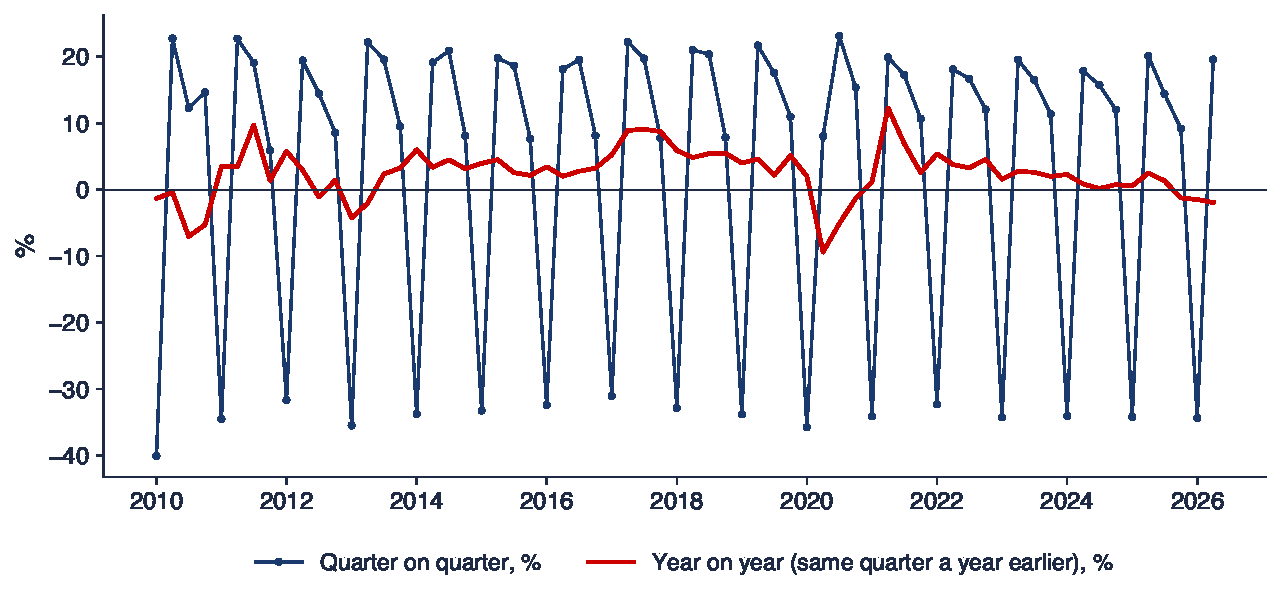
\includegraphics[width=0.94\textwidth,height=0.5\textheight,keepaspectratio]{ch0_sem_b1_growth.pdf}
\end{center}
\vspace{-2mm}
\begin{itemize}
    \item Blue: q/q swings between about $-35\%$ and $+20\%$ every year; red: y/y moves slowly, around the business cycle
    \item \textbf{Interpretation}: only the y/y rate shows the recessions (2009--2010, 2020) and the slowdown of 2025--2026; for unadjusted data, report y/y growth
\end{itemize}
\quantlet{TSA\_ch0\_seminar}{\qlurl{TSA_ch0_seminar}}
\end{frame}

\begin{frame}{B2 [Solved]: EUR/RON: Memory of Levels and Changes --- Task}
\itemsize{\footnotesize}
\begin{itemize}
\item \textbf{Question}: does today's exchange rate help to forecast tomorrow's, and does today's change help to forecast tomorrow's change?
\item \textbf{Inputs}: EUR/RON reference rate of the BNR, 5 January 2015 -- 18 September 2026 (2\,939 days)
\item \textbf{Tasks}
\begin{enumerate}
    \item Compute the daily log returns $r_t = 100\,(\ln P_t - \ln P_{t-1})$.
    \item Compute the sample ACF of the level and of the returns for lags 1--20.
    \item Compare $r_1$ of the returns with the band $\pm 1.96/\sqrt T$, and count the lags outside the band.
    \item Interpretation: is the naive forecast a sensible benchmark for the exchange rate?
\end{enumerate}
\item \textbf{Report}: $r_1$ and $r_{20}$ of the level, $r_1$ and $r_2$ of the returns, the band, the number of lags outside it, and the answer to the interpretation question
\item Notebook: section B2
\end{itemize}
\end{frame}

\begin{frame}{B2 [Solved]: Solution (1/2) --- Step by Step}
\itemsize{\footnotesize}
\begin{itemize}
    \item \textbf{Level}: $r_1 = $ 1.00, $r_{20} = $ 0.97
    \begin{itemize}
        \item the level remembers itself for weeks: a slow decay, the signature of a trend
    \end{itemize}
    \item \textbf{Returns}: standard deviation 0.13\% a day; $r_1 = $ 0.078, $r_2 = $ -0.0003
    \begin{itemize}
        \item band $\pm$0.036; 8 of the 20 lags lie outside it
        \item $r_1$ is significant but small: yesterday's change explains less than 1\% of the variance of today's change ($r_1^2$)
    \end{itemize}
\end{itemize}
\quantlet{TSA\_ch0\_seminar}{\qlurl{TSA_ch0_seminar}}
\end{frame}

\begin{frame}{B2 [Solved]: Solution (2/2) --- Chart and Interpretation}
\itemsize{\footnotesize}
\begin{center}
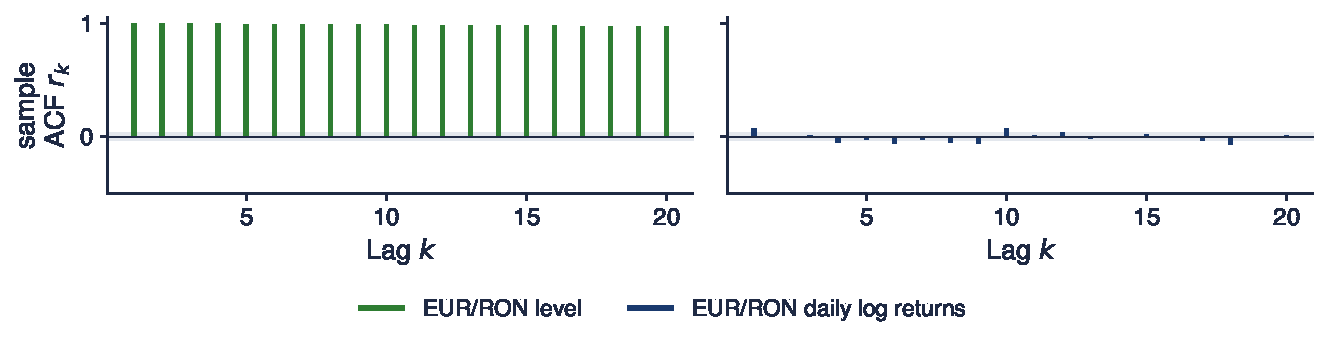
\includegraphics[width=0.94\textwidth,height=0.46\textheight,keepaspectratio]{ch0_sem_b2_acf.pdf}
\end{center}
\vspace{-2mm}
\begin{itemize}
    \item Left: the ACF of the level stays close to 1; right: the ACF of the returns is almost flat; shaded: the band $\pm 1.96/\sqrt T$
    \item \textbf{Interpretation}: yes; the level of today is the best simple forecast of tomorrow's level, while past changes add very little: the naive forecast is the benchmark to beat
\end{itemize}
\quantlet{TSA\_ch0\_seminar}{\qlurl{TSA_ch0_seminar}}
\end{frame}


%=============================================================================
\section{Your Turn}
%=============================================================================

\begin{frame}{A4 [Proposed]: New Numbers --- Task}
\itemsize{\footnotesize}
\begin{itemize}
\item \textbf{Question}: can you repeat A1--A3 without the solution in front of you?
\item \textbf{Inputs}: a quarterly series 120, 150, 132, 168, 126 (Q1 of year 1 to Q1 of year 2); a series 5, 7, 6, 8, 9; a series with $m = 3$: training 20, 30, 25, 22, 32, 27, test 23, 33, 29
\item \textbf{Tasks}
\begin{enumerate}
    \item Model: A1, A2 and A3 [Solved].
    \item Compute the period-on-period growth rates, the log differences and the year-on-year rate of the last quarter.
    \item Compute $r_1$ of the series 5, 7, 6, 8, 9 and the band $\pm 1.96/\sqrt T$.
    \item Compute the MAE and the RMSE of the naive and seasonal naive forecasts of the test values.
\end{enumerate}
\item \textbf{Report}: the growth table, $r_1$ and the band, the four error measures, and one sentence naming the better forecast
\item Notebook: section A4
\end{itemize}
\end{frame}

\ifsolutions
\begin{frame}{A4: Solution (Instructor)}
\itemsize{\footnotesize}
\begin{itemize}
    \item \textbf{Growth}
    \begin{itemize}
        \item period on period, \%: $+$25.0, -12.0, $+$27.3, -25.0; log differences: $+$22.3, -12.8, $+$24.1, -28.8
        \item year on year (Q1 of year 2): $100\,(126/120 - 1) = +$5.0\%
    \end{itemize}
    \item \textbf{Autocorrelation}: $\bar y = 7$, $\sum d^2 = 10$, $\sum d_t d_{t-1} = 1$
    \begin{itemize}
        \item $r_1 = $ 0.10; band $\pm$0.88: not distinguishable from 0
    \end{itemize}
    \item \textbf{Forecasts} (naive: 27, 27, 27; seasonal naive: 22, 32, 27)
    \begin{itemize}
        \item naive: MAE 4.00, RMSE 4.32; seasonal naive: MAE 1.33, RMSE 1.41; the seasonal naive wins
    \end{itemize}
\end{itemize}
\end{frame}
\fi

\begin{frame}{B3 [Proposed]: Romanian Inflation --- Task}
\itemsize{\footnotesize}
\begin{itemize}
\item \textbf{Question}: does monthly inflation have a seasonal pattern that the annual rate hides?
\item \textbf{Inputs}: Romanian HICP, 2015 = 100, monthly, 1 January 2015 -- 1 August 2026 (Eurostat)
\item \textbf{Tasks}
\begin{enumerate}
    \item Model: B1 and B2 [Solved].
    \item Compute the monthly (m/m) and the annual (y/y) inflation rates in \%.
    \item Compute the average monthly inflation for each calendar month.
    \item Compute the ACF of the monthly rate for lags 1--24, and of the annual rate at lag 1.
    \item Interpretation: why is the annual rate so persistent?
\end{enumerate}
\item \textbf{Report}: the latest monthly and annual rates, the months with the highest and lowest average, $r_1$ and $r_{12}$ of the monthly rate, $r_1$ of the annual rate, and the answer to the interpretation question
\item Notebook: section B3
\end{itemize}
\end{frame}

\ifsolutions
\begin{frame}{B3: Solution (Instructor)}
\itemsize{\footnotesize}
\begin{columns}[T]
\begin{column}{0.5\textwidth}
\begin{center}
\includegraphics[width=0.94\textwidth,height=0.42\textheight,keepaspectratio]{ch0_sem_b3_acf.pdf}
\end{center}
\vspace{-2mm}

\end{column}
\begin{column}{0.47\textwidth}
\begin{itemize}
    \item August 2026: monthly $+$0.3\%, annual 6.3\%; annual peak 14.6\% in November 2022
    \item highest average month: October (0.7\%); lowest: June (-0.1\%)
    \item monthly rate: $r_1 = $ 0.48, $r_{12} = $ 0.29 (band $\pm$0.17): memory and a seasonal peak
    \item annual rate: $r_1 = $ 0.98: two consecutive annual rates share 11 of their 12 monthly changes (as in Slutsky's moving sums)
\end{itemize}
\end{column}
\end{columns}
\end{frame}
\fi

\begin{frame}{B4 [Proposed]: Electricity: Naive or Seasonal Naive? --- Task}
\itemsize{\footnotesize}
\begin{itemize}
\item \textbf{Question}: for monthly electricity generation, does the seasonal naive forecast beat the naive one?
\item \textbf{Inputs}: net electricity generation in Romania, TWh per month (Eurostat); test set: August 2024 -- July 2026 (24 months)
\item \textbf{Tasks}
\begin{enumerate}
    \item Model: A3 [Solved].
    \item Split the series by time: the last 24 months form the test set.
    \item Forecast the test set with the naive and with the seasonal naive method ($m = 12$), using only the training set.
    \item Compute the MAE and the RMSE of each method, and plot both forecasts against the test data.
    \item Interpretation: why does the seasonal naive method not win clearly here?
\end{enumerate}
\item \textbf{Report}: the four error measures, the chart, and the answer to the interpretation question
\item Notebook: section B4
\end{itemize}
\end{frame}

\ifsolutions
\begin{frame}{B4: Solution (Instructor)}
\itemsize{\footnotesize}
\begin{columns}[T]
\begin{column}{0.5\textwidth}
\begin{center}
\includegraphics[width=0.94\textwidth,height=0.42\textheight,keepaspectratio]{ch0_sem_b4_forecast.pdf}
\end{center}
\vspace{-2mm}

\end{column}
\begin{column}{0.47\textwidth}
\begin{itemize}
    \item naive (all forecasts 3.97 TWh): MAE 0.28, RMSE 0.33
    \item seasonal naive: MAE 0.28, RMSE 0.38
    \item the two are almost equal: the seasonal naive copies the strong winter of the training year into a lower test period, so its winter errors are large
    \item a method that combines season and level (Holt--Winters, in the lecture) does better
\end{itemize}
\end{column}
\end{columns}
\end{frame}
\fi


%=============================================================================
\section{Part C: Open Questions}
%=============================================================================

\begin{frame}{C1: A Project Idea}
\itemsize{\small}
\begin{itemize}
    \item \textbf{Question}: how much of the variation of a Romanian monthly series is seasonal, and is the seasonal pattern changing?
    \item \textbf{Candidate series} (Eurostat or INS)
    \begin{itemize}
        \item electricity generation, tourist arrivals, retail trade, industrial production
    \end{itemize}
    \item \textbf{Steps}
    \begin{itemize}
        \item plot the series and its year-on-year growth
        \item compare the average of each calendar month in the first and in the last five years
        \item after the lecture: decompose the series with STL and compare the seasonal amplitude over time
    \end{itemize}
    \item A good first step for the team project of \tsachlink{https://danpele.github.io/Time-Series-Analysis/EN/Courses/chapter0_introduction.pdf}{Chapters 0} and \tsachlink{https://danpele.github.io/Time-Series-Analysis/EN/Courses/chapter4_seasonality_forecasting.pdf}{4}
\end{itemize}
\end{frame}

\begin{frame}[fragile]{C2 [Proposed]: Critique an AI Answer --- the Answer}
\itemsize{\footnotesize}
\begin{itemize}
    \item \textbf{Prompt} sent to an AI assistant: ``From the quarterly Romanian real GDP, compute the average annual growth rate and the RMSE of a naive forecast.''
\end{itemize}
\begin{lstlisting}
g = read_eurostat('namq_10_gdp', 'Q.CLV10_MEUR.NSA.B1GQ.RO') / 1000
growth = g.diff()                                # annual growth rate, %
print('average annual growth:', growth.mean())
test = g.sample(frac=0.2, random_state=1).sort_index()   # test set
train = g.drop(test.index)                               # training set
fc = train.reindex(g.index).ffill().shift(1).reindex(test.index)  # naive
rmse = ((test - fc) ** 2).mean()
print('RMSE of the naive forecast:', rmse)
\end{lstlisting}
\begin{itemize}
    \item \textbf{Conclusion of the AI}: ``Romanian GDP grows by only 0.24\% a year, and the naive forecast has an RMSE of 111.9 billion EUR, larger than GDP itself: forecasting GDP is hopeless.''
\end{itemize}
\end{frame}

\begin{frame}{C2 [Proposed]: Critique an AI Answer --- Task}
\itemsize{\small}
\begin{itemize}
\item \textbf{Question}: can you trust code that runs without an error message?
\item \textbf{Inputs}: the code and the conclusion on the previous slide; the definitions of the primer
\item \textbf{Tasks}
\begin{enumerate}
    \item Model: A1, A3 and B1 [Solved].
    \item Find the three errors planted in the code.
    \item For each error, say how you would detect it: a check on the output, the primer, or a solved exercise.
    \item Write the corrected code, with the last 8 quarters as the test set, and report the corrected numbers.
    \item Say whether the conclusion ``forecasting GDP is hopeless'' survives.
\end{enumerate}
\item \textbf{Report}: one line per error in the format: request, answer, error, how found, correction; the corrected growth and RMSE
\item Notebook: section C2
\end{itemize}
\end{frame}

\ifsolutions
\begin{frame}{C2: Solution (Instructor)}
\itemsize{\footnotesize}
\begin{itemize}
    \item \textbf{Error 1}: \texttt{g.diff()} is a change in billion EUR over one quarter, not an annual growth rate in \%
    \begin{itemize}
        \item detect: units (A1, B1); correct: \texttt{100 * (g / g.shift(4) - 1)}, average 2.9\% a year
    \end{itemize}
    \item \textbf{Error 2}: a random test set; earlier test quarters are forecast with later data
    \begin{itemize}
        \item detect: the primer (split by time); correct: \texttt{train, test = g.iloc[:-8], g.iloc[-8:]}
    \end{itemize}
    \item \textbf{Error 3}: the mean squared error without the square root, in (billion EUR)$^2$
    \begin{itemize}
        \item detect: an RMSE larger than the series itself (A3); correct: \texttt{np.sqrt(...)}
    \end{itemize}
    \item Corrected, last 8 quarters: RMSE 8.36 billion EUR (naive), 0.56 (seasonal naive): the conclusion fails; a seasonal benchmark forecasts GDP within about 1\%
\end{itemize}
\end{frame}
\fi


%=============================================================================
\section{Wrap-up}
%=============================================================================

\begin{frame}{Practice at Home}
\itemsize{\small}
\begin{itemize}
    \item \textbf{Finish the proposed exercises}: A4, B3, B4 and C2
    \begin{itemize}
        \item each names its model, a solved exercise to follow
    \end{itemize}
    \item \textbf{Try one more series}
    \begin{itemize}
        \item repeat B1 for the euro area GDP (key \texttt{Q.CLV10\_MEUR.NSA.B1GQ.EA20}) and compare the seasonal swings with Romania
    \end{itemize}
    \item \textbf{Take the \tsachlink{https://danpele.github.io/Time-Series-Analysis/EN/Courses/chapter0_introduction.pdf}{Chapter 0} quiz} on the course website: 20 questions, each answer explained
\end{itemize}
\end{frame}

\begin{frame}{Recap, and Next: the \tsachlinkt{https://danpele.github.io/Time-Series-Analysis/EN/Courses/chapter0_introduction.pdf}{Chapter 0} Lecture}
\itemsize{\footnotesize}
\begin{columns}[T]
\begin{column}{0.52\textwidth}
\begin{itemize}
    \item \textbf{Today}
    \begin{itemize}
        \item for unadjusted data, report growth over a year, not over one quarter
        \item $r_k$: how much a series remembers its value $k$ periods earlier
        \item levels with a trend remember a lot; daily changes of prices remember little
        \item the naive and seasonal naive forecasts are the benchmarks; split by time, then measure MAE and RMSE
        \item AI code can run and still be wrong
    \end{itemize}
\end{itemize}
\end{column}
\begin{column}{0.45\textwidth}
\begin{itemize}
    \item \textbf{In the lecture}
    \begin{itemize}
        \item How is the course organised and graded?
        \item Which components make up a time series?
        \item How does exponential smoothing forecast?
        \item Which forecasts win on real Romanian data?
    \end{itemize}
    \item The seminar is practice and is not graded; the solutions of the [Proposed] tasks are discussed in class
\end{itemize}
\end{column}
\end{columns}
\end{frame}

\end{document}
